% Options for packages loaded elsewhere
\PassOptionsToPackage{unicode}{hyperref}
\PassOptionsToPackage{hyphens}{url}
%
\documentclass[
  american,
  man,floatsintext]{apa7}
\usepackage{amsmath,amssymb}
\usepackage{lmodern}
\usepackage{ifxetex,ifluatex}
\ifnum 0\ifxetex 1\fi\ifluatex 1\fi=0 % if pdftex
  \usepackage[T1]{fontenc}
  \usepackage[utf8]{inputenc}
  \usepackage{textcomp} % provide euro and other symbols
\else % if luatex or xetex
  \usepackage{unicode-math}
  \defaultfontfeatures{Scale=MatchLowercase}
  \defaultfontfeatures[\rmfamily]{Ligatures=TeX,Scale=1}
\fi
% Use upquote if available, for straight quotes in verbatim environments
\IfFileExists{upquote.sty}{\usepackage{upquote}}{}
\IfFileExists{microtype.sty}{% use microtype if available
  \usepackage[]{microtype}
  \UseMicrotypeSet[protrusion]{basicmath} % disable protrusion for tt fonts
}{}
\makeatletter
\@ifundefined{KOMAClassName}{% if non-KOMA class
  \IfFileExists{parskip.sty}{%
    \usepackage{parskip}
  }{% else
    \setlength{\parindent}{0pt}
    \setlength{\parskip}{6pt plus 2pt minus 1pt}}
}{% if KOMA class
  \KOMAoptions{parskip=half}}
\makeatother
\usepackage{xcolor}
\IfFileExists{xurl.sty}{\usepackage{xurl}}{} % add URL line breaks if available
\IfFileExists{bookmark.sty}{\usepackage{bookmark}}{\usepackage{hyperref}}
\hypersetup{
  pdftitle={Supplementary Materials: Cognitive Load and Moral Dumbfounding},
  pdfauthor={Cillian McHugh1, Marek McGann2, Eric R. Igou1, \& Elaine L Kinsella1},
  pdflang={en-US},
  pdfkeywords={keywords},
  hidelinks,
  pdfcreator={LaTeX via pandoc}}
\urlstyle{same} % disable monospaced font for URLs
\usepackage{graphicx}
\makeatletter
\def\maxwidth{\ifdim\Gin@nat@width>\linewidth\linewidth\else\Gin@nat@width\fi}
\def\maxheight{\ifdim\Gin@nat@height>\textheight\textheight\else\Gin@nat@height\fi}
\makeatother
% Scale images if necessary, so that they will not overflow the page
% margins by default, and it is still possible to overwrite the defaults
% using explicit options in \includegraphics[width, height, ...]{}
\setkeys{Gin}{width=\maxwidth,height=\maxheight,keepaspectratio}
% Set default figure placement to htbp
\makeatletter
\def\fps@figure{htbp}
\makeatother
\setlength{\emergencystretch}{3em} % prevent overfull lines
\providecommand{\tightlist}{%
  \setlength{\itemsep}{0pt}\setlength{\parskip}{0pt}}
\setcounter{secnumdepth}{-\maxdimen} % remove section numbering
% Make \paragraph and \subparagraph free-standing
\ifx\paragraph\undefined\else
  \let\oldparagraph\paragraph
  \renewcommand{\paragraph}[1]{\oldparagraph{#1}\mbox{}}
\fi
\ifx\subparagraph\undefined\else
  \let\oldsubparagraph\subparagraph
  \renewcommand{\subparagraph}[1]{\oldsubparagraph{#1}\mbox{}}
\fi
% Manuscript styling
\usepackage{upgreek}
\captionsetup{font=singlespacing,justification=justified}

% Table formatting
\usepackage{longtable}
\usepackage{lscape}
% \usepackage[counterclockwise]{rotating}   % Landscape page setup for large tables
\usepackage{multirow}		% Table styling
\usepackage{tabularx}		% Control Column width
\usepackage[flushleft]{threeparttable}	% Allows for three part tables with a specified notes section
\usepackage{threeparttablex}            % Lets threeparttable work with longtable

% Create new environments so endfloat can handle them
% \newenvironment{ltable}
%   {\begin{landscape}\begin{center}\begin{threeparttable}}
%   {\end{threeparttable}\end{center}\end{landscape}}
\newenvironment{lltable}{\begin{landscape}\begin{center}\begin{ThreePartTable}}{\end{ThreePartTable}\end{center}\end{landscape}}

% Enables adjusting longtable caption width to table width
% Solution found at http://golatex.de/longtable-mit-caption-so-breit-wie-die-tabelle-t15767.html
\makeatletter
\newcommand\LastLTentrywidth{1em}
\newlength\longtablewidth
\setlength{\longtablewidth}{1in}
\newcommand{\getlongtablewidth}{\begingroup \ifcsname LT@\roman{LT@tables}\endcsname \global\longtablewidth=0pt \renewcommand{\LT@entry}[2]{\global\advance\longtablewidth by ##2\relax\gdef\LastLTentrywidth{##2}}\@nameuse{LT@\roman{LT@tables}} \fi \endgroup}

% \setlength{\parindent}{0.5in}
% \setlength{\parskip}{0pt plus 0pt minus 0pt}

% Overwrite redefinition of paragraph and subparagraph by the default LaTeX template
% See https://github.com/crsh/papaja/issues/292
\makeatletter
\renewcommand{\paragraph}{\@startsection{paragraph}{4}{\parindent}%
  {0\baselineskip \@plus 0.2ex \@minus 0.2ex}%
  {-1em}%
  {\normalfont\normalsize\bfseries\itshape\typesectitle}}

\renewcommand{\subparagraph}[1]{\@startsection{subparagraph}{5}{1em}%
  {0\baselineskip \@plus 0.2ex \@minus 0.2ex}%
  {-\z@\relax}%
  {\normalfont\normalsize\itshape\hspace{\parindent}{#1}\textit{\addperi}}{\relax}}
\makeatother

% \usepackage{etoolbox}
\makeatletter
\patchcmd{\HyOrg@maketitle}
  {\section{\normalfont\normalsize\abstractname}}
  {\section*{\normalfont\normalsize\abstractname}}
  {}{\typeout{Failed to patch abstract.}}
\patchcmd{\HyOrg@maketitle}
  {\section{\protect\normalfont{\@title}}}
  {\section*{\protect\normalfont{\@title}}}
  {}{\typeout{Failed to patch title.}}
\makeatother
\keywords{keywords\newline\indent Word count: TBC}
\DeclareDelayedFloatFlavor{ThreePartTable}{table}
\DeclareDelayedFloatFlavor{lltable}{table}
\DeclareDelayedFloatFlavor*{longtable}{table}
\makeatletter
\renewcommand{\efloat@iwrite}[1]{\immediate\expandafter\protected@write\csname efloat@post#1\endcsname{}}
\makeatother
\usepackage{csquotes}
\usepackage[titles]{tocloft}
\cftpagenumbersoff{figure}
\renewcommand{\cftfigpresnum}{\itshape\figurename\enspace}
\renewcommand{\cftfigaftersnum}{.\space}
\setlength{\cftfigindent}{0pt}
\setlength{\cftafterloftitleskip}{0pt}
\settowidth{\cftfignumwidth}{Figure 10.\qquad}
\cftpagenumbersoff{table}
\renewcommand{\cfttabpresnum}{\itshape\tablename\enspace}
\renewcommand{\cfttabaftersnum}{.\space}
\setlength{\cfttabindent}{0pt}
\setlength{\cftafterloftitleskip}{0pt}
\settowidth{\cfttabnumwidth}{Table 10.\qquad}
\usepackage{float}
\ifxetex
  % Load polyglossia as late as possible: uses bidi with RTL langages (e.g. Hebrew, Arabic)
  \usepackage{polyglossia}
  \setmainlanguage[variant=american]{english}
\else
  \usepackage[main=american]{babel}
% get rid of language-specific shorthands (see #6817):
\let\LanguageShortHands\languageshorthands
\def\languageshorthands#1{}
\fi
\ifluatex
  \usepackage{selnolig}  % disable illegal ligatures
\fi

\title{Supplementary Materials: Cognitive Load and Moral Dumbfounding}
\author{Cillian McHugh\textsuperscript{1}, Marek McGann\textsuperscript{2}, Eric R. Igou\textsuperscript{1}, \& Elaine L Kinsella\textsuperscript{1}}
\date{}


\shorttitle{Cognitive Load and Moral Dumbfounding}

\authornote{

Correspondence concerning this article should be addressed to Cillian McHugh, University of Limerick, Limerick, Ireland, V94 T9PX. E-mail: \href{mailto:cillian.mchugh@ul.ie}{\nolinkurl{cillian.mchugh@ul.ie}}

}

\affiliation{\vspace{0.5cm}\textsuperscript{1} University of Limerick\\\textsuperscript{2} Mary Immaculate College \textasciitilde{} University of Limerick}

\abstract{
Six studies etc.
}



\begin{document}
\maketitle

\newpage

\hypertarget{list-of-tables}{%
\section{List of Tables}\label{list-of-tables}}

\newpage

\newpage

\begin{table}[tbp]

\begin{center}
\begin{threeparttable}

\caption{\label{tab:tabS1change}Study 1 – Changes in Jugment}

\begin{tabular}{ccc}
\toprule
Initial Judgment & \multicolumn{1}{c}{Revised Judgment} & \multicolumn{1}{c}{Total Changed}\\
\midrule
neutral & right & 1\\
neutral & wrong & 3\\
wrong & neutral & 7\\
wrong & right & 1\\
\bottomrule
\end{tabular}

\end{threeparttable}
\end{center}

\end{table}

\begin{table}[tbp]

\begin{center}
\begin{threeparttable}

\caption{\label{tab:tabS1tab1dumb1all}Study 1 – Response to the critical slide depending on cognitive load}

\begin{tabular}{lcccc}
\toprule
 & \multicolumn{2}{c}{Cognitive Load} & \multicolumn{2}{c}{Control} \\
\cmidrule(r){2-3} \cmidrule(r){4-5}
 & \multicolumn{1}{c}{N} & \multicolumn{1}{c}{\%} & \multicolumn{1}{c}{N} & \multicolumn{1}{c}{\%}\\
\midrule
It's wrong and I can provide a valid reason. & 12 & 36\% & 21 & 64\%\\
It's wrong but I can't think of a reason. & 6 & 18\% & 7 & 21\%\\
There is nothing wrong. & 15 & 45\% & 5 & 15\%\\
\bottomrule
\end{tabular}

\end{threeparttable}
\end{center}

\end{table}

\newpage

\newpage

\begin{table}[tbp]

\begin{center}
\begin{threeparttable}

\caption{\label{tab:tabS6change}Study 6 – Changes in Jugment (full sample)}

\begin{tabular}{ccc}
\toprule
Initial Judgment & \multicolumn{1}{c}{Revised Judgment} & \multicolumn{1}{c}{Total Changed}\\
\midrule
neutral & right & 8\\
neutral & wrong & 19\\
right & neutral & 10\\
right & wrong & 61\\
wrong & neutral & 29\\
wrong & right & 73\\
\bottomrule
\end{tabular}

\end{threeparttable}
\end{center}

\end{table}

\newpage

\begin{table}[tbp]

\begin{center}
\begin{threeparttable}

\caption{\label{tab:tabS6changeeachscenario}Study 6 – Changes in Jugment for each Scenario}

\begin{tabular}{lccc}
\toprule
Scenario & \multicolumn{1}{c}{Initial Judgment} & \multicolumn{1}{c}{Revised Judgment} & \multicolumn{1}{c}{Total Changed}\\
\midrule
Julie and Mark & neutral & right & 1\\
 & neutral & wrong & 4\\
 & right & wrong & 6\\
 & wrong & neutral & 9\\
 & wrong & right & 8\\
Jennifer & neutral & right & 1\\
 & neutral & wrong & 3\\
 & right & neutral & 2\\
 & right & wrong & 10\\
 & wrong & neutral & 2\\
 & wrong & right & 11\\
Trolley & neutral & right & 4\\
 & neutral & wrong & 7\\
 & right & neutral & 4\\
 & right & wrong & 18\\
 & wrong & neutral & 14\\
 & wrong & right & 26\\
Heinz & neutral & right & 2\\
 & neutral & wrong & 5\\
 & right & neutral & 4\\
 & right & wrong & 27\\
 & wrong & neutral & 4\\
 & wrong & right & 28\\
\bottomrule
\end{tabular}

\end{threeparttable}
\end{center}

\end{table}

\newpage

\begin{table}[tbp]

\begin{center}
\begin{threeparttable}

\caption{\label{tab:tabS6tab1dumb1all}Study 6 – Response to the critical slide depending on cognitive load (full sample)}

\begin{tabular}{lcccc}
\toprule
 & \multicolumn{2}{c}{Cognitive Load} & \multicolumn{2}{c}{Control} \\
\cmidrule(r){2-3} \cmidrule(r){4-5}
 & \multicolumn{1}{c}{N} & \multicolumn{1}{c}{\%} & \multicolumn{1}{c}{N} & \multicolumn{1}{c}{\%}\\
\midrule
It's wrong and I can provide a valid reason. & 113 & 56\% & 143 & 67\%\\
It's wrong but I can't think of a reason. & 55 & 27\% & 36 & 17\%\\
There is nothing wrong. & 35 & 17\% & 36 & 17\%\\
\bottomrule
\end{tabular}

\end{threeparttable}
\end{center}

\end{table}

\newpage

\newpage

\newpage

\newpage

\begin{table}[tbp]

\begin{center}
\begin{threeparttable}

\caption{\label{tab:tabS6tab1dumb1allIncest}Study 6 – Response to the critical slide depending on cognitive load, for each scenario}

\begin{tabular}{llcccc}
\toprule
 &  & \multicolumn{2}{c}{Cognitive Load} & \multicolumn{2}{c}{Control} \\
\cmidrule(r){3-4} \cmidrule(r){5-6}
Scenario & \multicolumn{1}{c}{Response} & \multicolumn{1}{c}{N} & \multicolumn{1}{c}{\%} & \multicolumn{1}{c}{N} & \multicolumn{1}{c}{\%}\\
\midrule
Julie and Mark & Reasons & 106 & 54\% & 123 & 57\%\\
 & Dumbfounded & 51 & 26\% & 51 & 24\%\\
 & Nothing Wrong & 40 & 20\% & 41 & 19\%\\
Jennifer & Reasons & 142 & 65\% & 173 & 81\%\\
 & Dumbfounded & 67 & 31\% & 30 & 14\%\\
 & Nothing Wrong & 9 & 4\% & 11 & 5\%\\
Trolley & Reasons & 97 & 47\% & 135 & 62\%\\
 & Dumbfounded & 72 & 35\% & 55 & 25\%\\
 & Nothing Wrong & 39 & 19\% & 26 & 12\%\\
Heinz & Reasons & 113 & 56\% & 143 & 67\%\\
 & Dumbfounded & 55 & 27\% & 36 & 17\%\\
 & Nothing Wrong & 35 & 17\% & 36 & 17\%\\
\bottomrule
\end{tabular}

\end{threeparttable}
\end{center}

\end{table}

\newpage

\newpage

\begin{table}[tbp]

\begin{center}
\begin{threeparttable}

\caption{\label{tab:tabS6tab1dumbIncest}Study 6 – Observed counts, expected counts, and standardised residuals for each response to the critical slide depending on cognitive load (Julie and Mark)}

\begin{tabular}{llcc}
\toprule
 & \multicolumn{1}{c}{} & \multicolumn{1}{c}{Cognitive Load} & \multicolumn{1}{c}{Control}\\
\midrule
Observed count & Reasons & 106.00 & 123.00\\
 & Dumbfounded & 51.00 & 51.00\\
 & Nothing Wrong & 40.00 & 41.00\\
Expected count & Reasons & 109.50 & 119.50\\
 & Dumbfounded & 48.77 & 53.23\\
 & Nothing Wrong & 38.73 & 42.27\\
Standardised residuals & Reasons & -0.69 & 0.69\\
 & Dumbfounded & 0.51 & -0.51\\
 & Nothing Wrong & 0.32 & -0.32\\
\bottomrule
\addlinespace
\end{tabular}

\begin{tablenotes}[para]
\normalsize{\textit{Note.} * = sig. at \emph{p} < .05; ** = sig. at \emph{p} < .001}
\end{tablenotes}

\end{threeparttable}
\end{center}

\end{table}

\newpage

\newpage

\begin{table}[tbp]

\begin{center}
\begin{threeparttable}

\caption{\label{tab:tabS6tab1dumbJennifer}Study 6 – Observed counts, expected counts, and standardised residuals for each response to the critical slide depending on cognitive load (Jennifer)}

\begin{tabular}{llcc}
\toprule
 & \multicolumn{1}{c}{} & \multicolumn{1}{c}{Cognitive Load} & \multicolumn{1}{c}{Control}\\
\midrule
Observed count & Reasons & 142 & 173\\
 & Dumbfounded & 67 & 30\\
 & Nothing Wrong & 9 & 11\\
Expected count & Reasons & 158.96 & 156.04\\
 & Dumbfounded & 48.95 & 48.05\\
 & Nothing Wrong & 10.09 & 9.91\\
Standardised residuals & Reasons & -3.67** & 3.67**\\
 & Dumbfounded & 4.16** & -4.16**\\
 & Nothing Wrong & -0.5 & 0.5\\
\bottomrule
\addlinespace
\end{tabular}

\begin{tablenotes}[para]
\normalsize{\textit{Note.} * = sig. at \emph{p} < .05; ** = sig. at \emph{p} < .001}
\end{tablenotes}

\end{threeparttable}
\end{center}

\end{table}

\newpage

\newpage

\begin{table}[tbp]

\begin{center}
\begin{threeparttable}

\caption{\label{tab:tabS6tab1dumbTrolley}Study 6 – Observed counts, expected counts, and standardised residuals for each response to the critical slide depending on cognitive load (Trolley)}

\begin{tabular}{llcc}
\toprule
 & \multicolumn{1}{c}{} & \multicolumn{1}{c}{Cognitive Load} & \multicolumn{1}{c}{Control}\\
\midrule
Observed count & Reasons & 97 & 135\\
 & Dumbfounded & 72 & 55\\
 & Nothing Wrong & 39 & 26\\
Expected count & Reasons & 113.81 & 118.19\\
 & Dumbfounded & 62.3 & 64.7\\
 & Nothing Wrong & 31.89 & 33.11\\
Standardised residuals & Reasons & -3.28* & 3.28*\\
 & Dumbfounded & 2.06* & -2.06*\\
 & Nothing Wrong & 1.92 & -1.92\\
\bottomrule
\addlinespace
\end{tabular}

\begin{tablenotes}[para]
\normalsize{\textit{Note.} * = sig. at \emph{p} < .05; ** = sig. at \emph{p} < .001}
\end{tablenotes}

\end{threeparttable}
\end{center}

\end{table}

\newpage

\newpage

\begin{table}[tbp]

\begin{center}
\begin{threeparttable}

\caption{\label{tab:tabS6tab1dumbHeinz}Study 6 – Observed counts, expected counts, and standardised residuals for each response to the critical slide depending on cognitive load (Heinz)}

\begin{tabular}{llcc}
\toprule
 & \multicolumn{1}{c}{} & \multicolumn{1}{c}{Cognitive Load} & \multicolumn{1}{c}{Control}\\
\midrule
Observed count & Reasons & 113 & 143\\
 & Dumbfounded & 55 & 36\\
 & Nothing Wrong & 35 & 36\\
Expected count & Reasons & 124.33 & 131.67\\
 & Dumbfounded & 44.19 & 46.81\\
 & Nothing Wrong & 34.48 & 36.52\\
Standardised residuals & Reasons & -2.27* & 2.27*\\
 & Dumbfounded & 2.56* & -2.56*\\
 & Nothing Wrong & 0.14 & -0.14\\
\bottomrule
\addlinespace
\end{tabular}

\begin{tablenotes}[para]
\normalsize{\textit{Note.} * = sig. at \emph{p} < .05; ** = sig. at \emph{p} < .001}
\end{tablenotes}

\end{threeparttable}
\end{center}

\end{table}

\newpage

\newpage

\newpage

\hypertarget{list-of-figures}{%
\section{List of Figures}\label{list-of-figures}}

\newpage
\newpage

\newpage

\begin{figure}[!p]
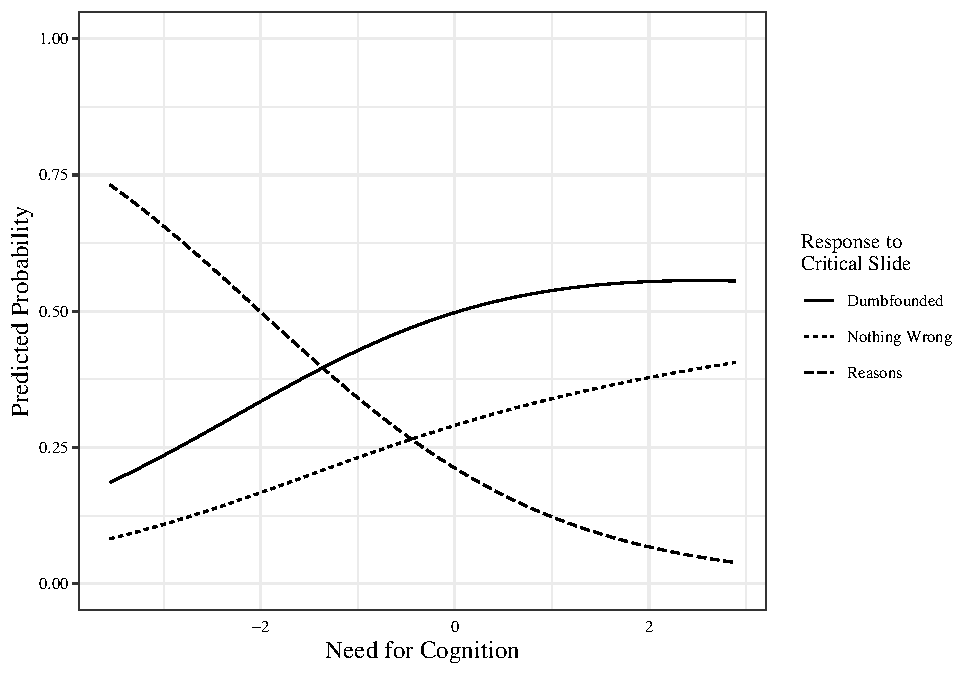
\includegraphics{Supplementary_files/figure-latex/figggplotlogit1-1} \caption{Study 1: Probability of selecting each response to the critical slide depending on Need for Cognition}\label{fig:figggplotlogit1}
\end{figure}

\newpage

\begin{figure}[!p]
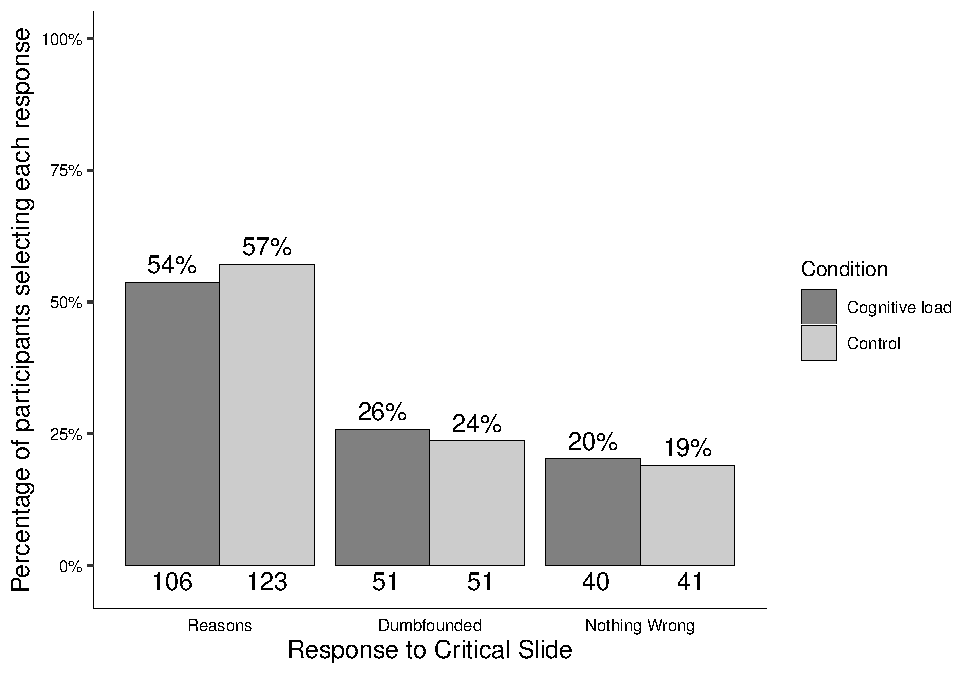
\includegraphics{Supplementary_files/figure-latex/figS6ch5S6fig2criticalconditionbIncest-1} \caption{Study 6: Responses to critical slide depending on cognitive load (Julie and Mark)}\label{fig:figS6ch5S6fig2criticalconditionbIncest}
\end{figure}

\begin{figure}[!p]
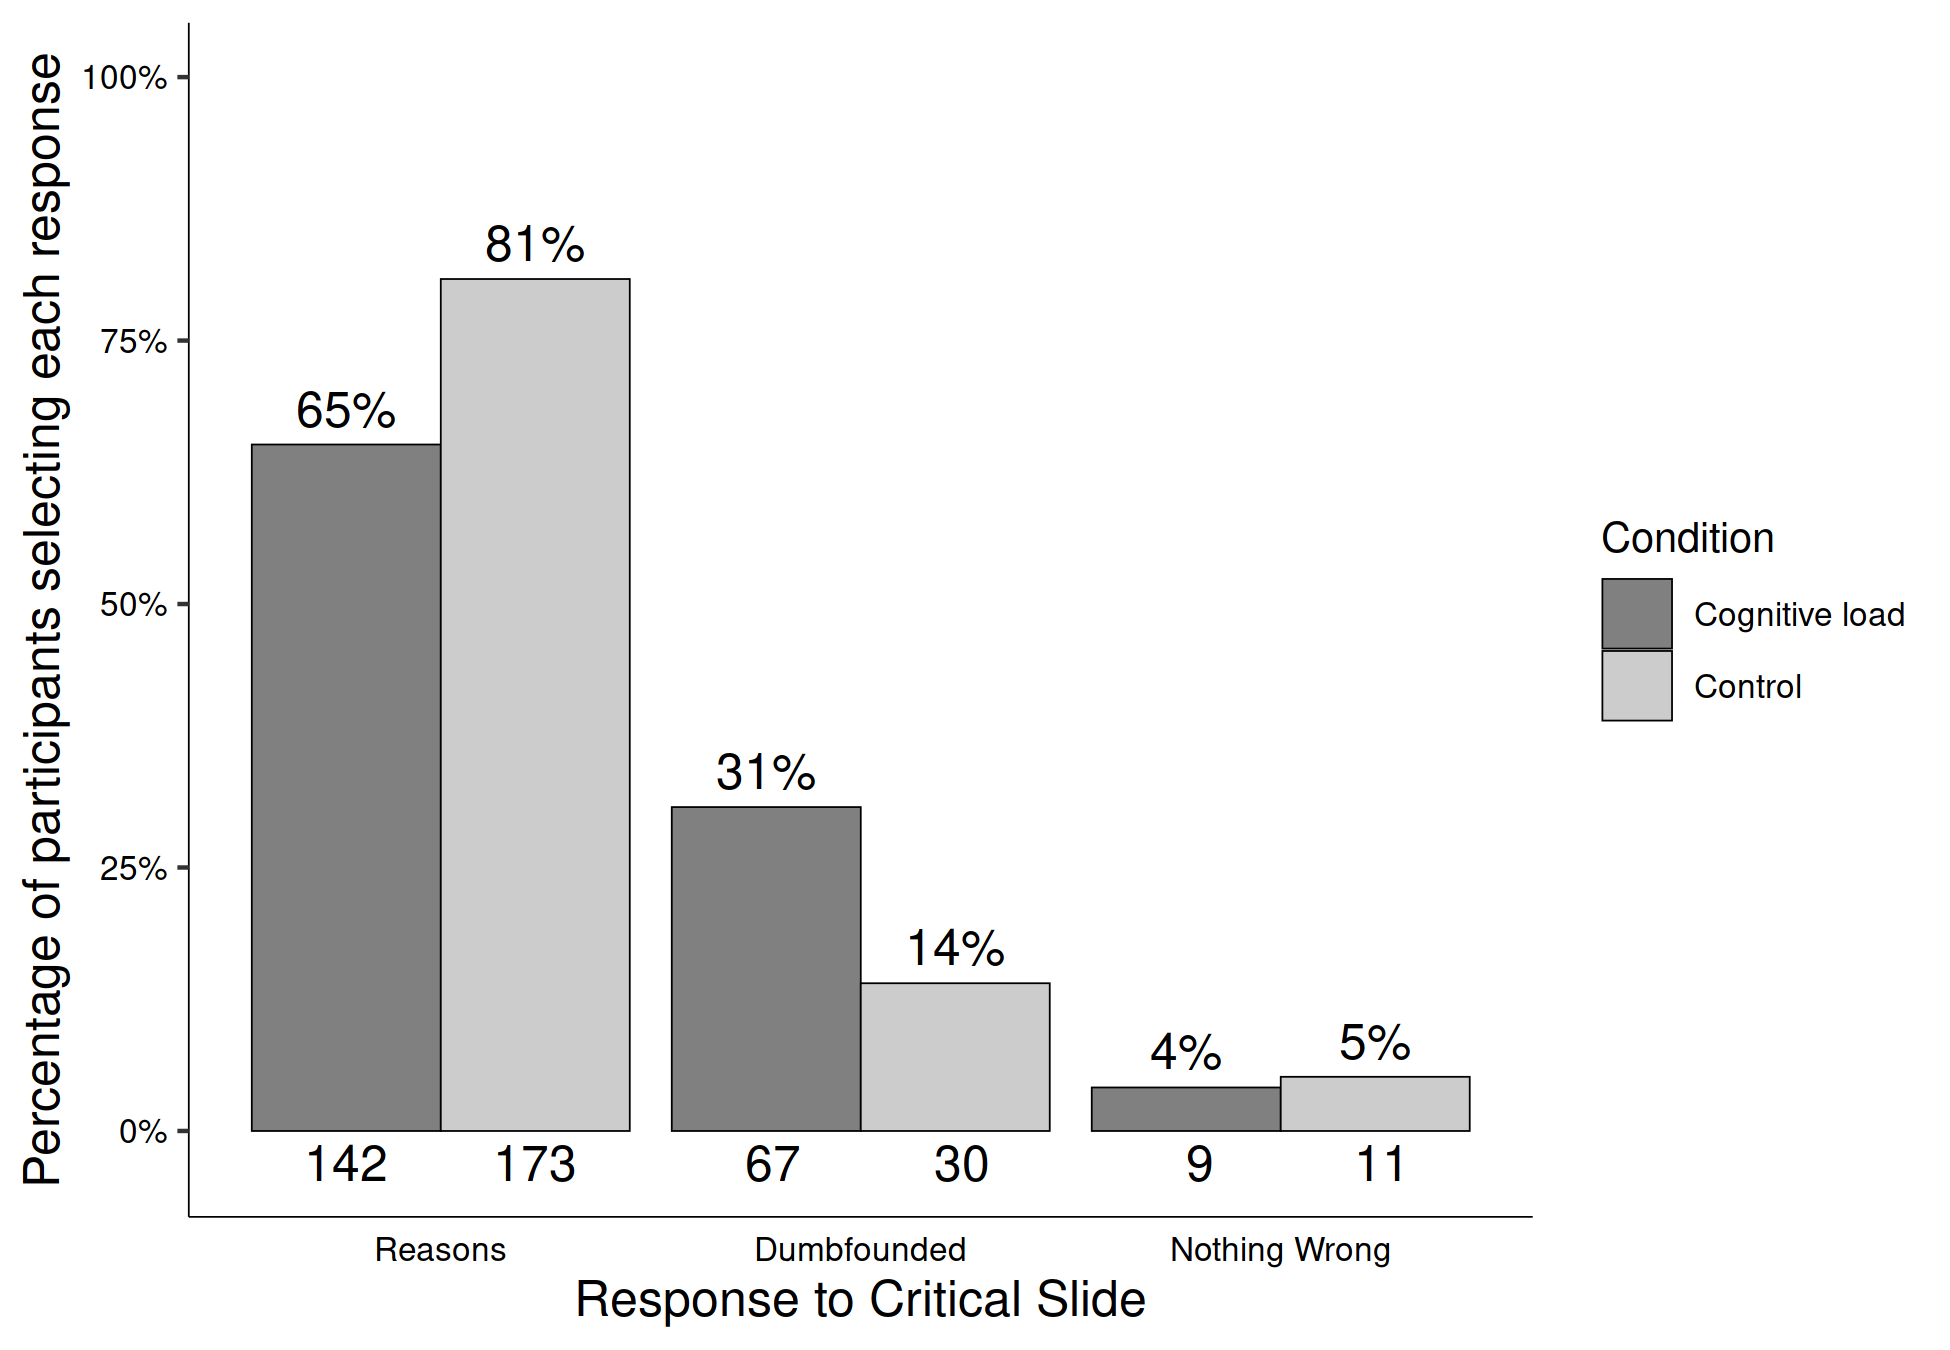
\includegraphics{Supplementary_files/figure-latex/figS6ch5S6fig2criticalconditionbJennifer-1} \caption{Study 6: Responses to critical slide depending on cognitive load (Jennifer)}\label{fig:figS6ch5S6fig2criticalconditionbJennifer}
\end{figure}

\begin{figure}[!p]
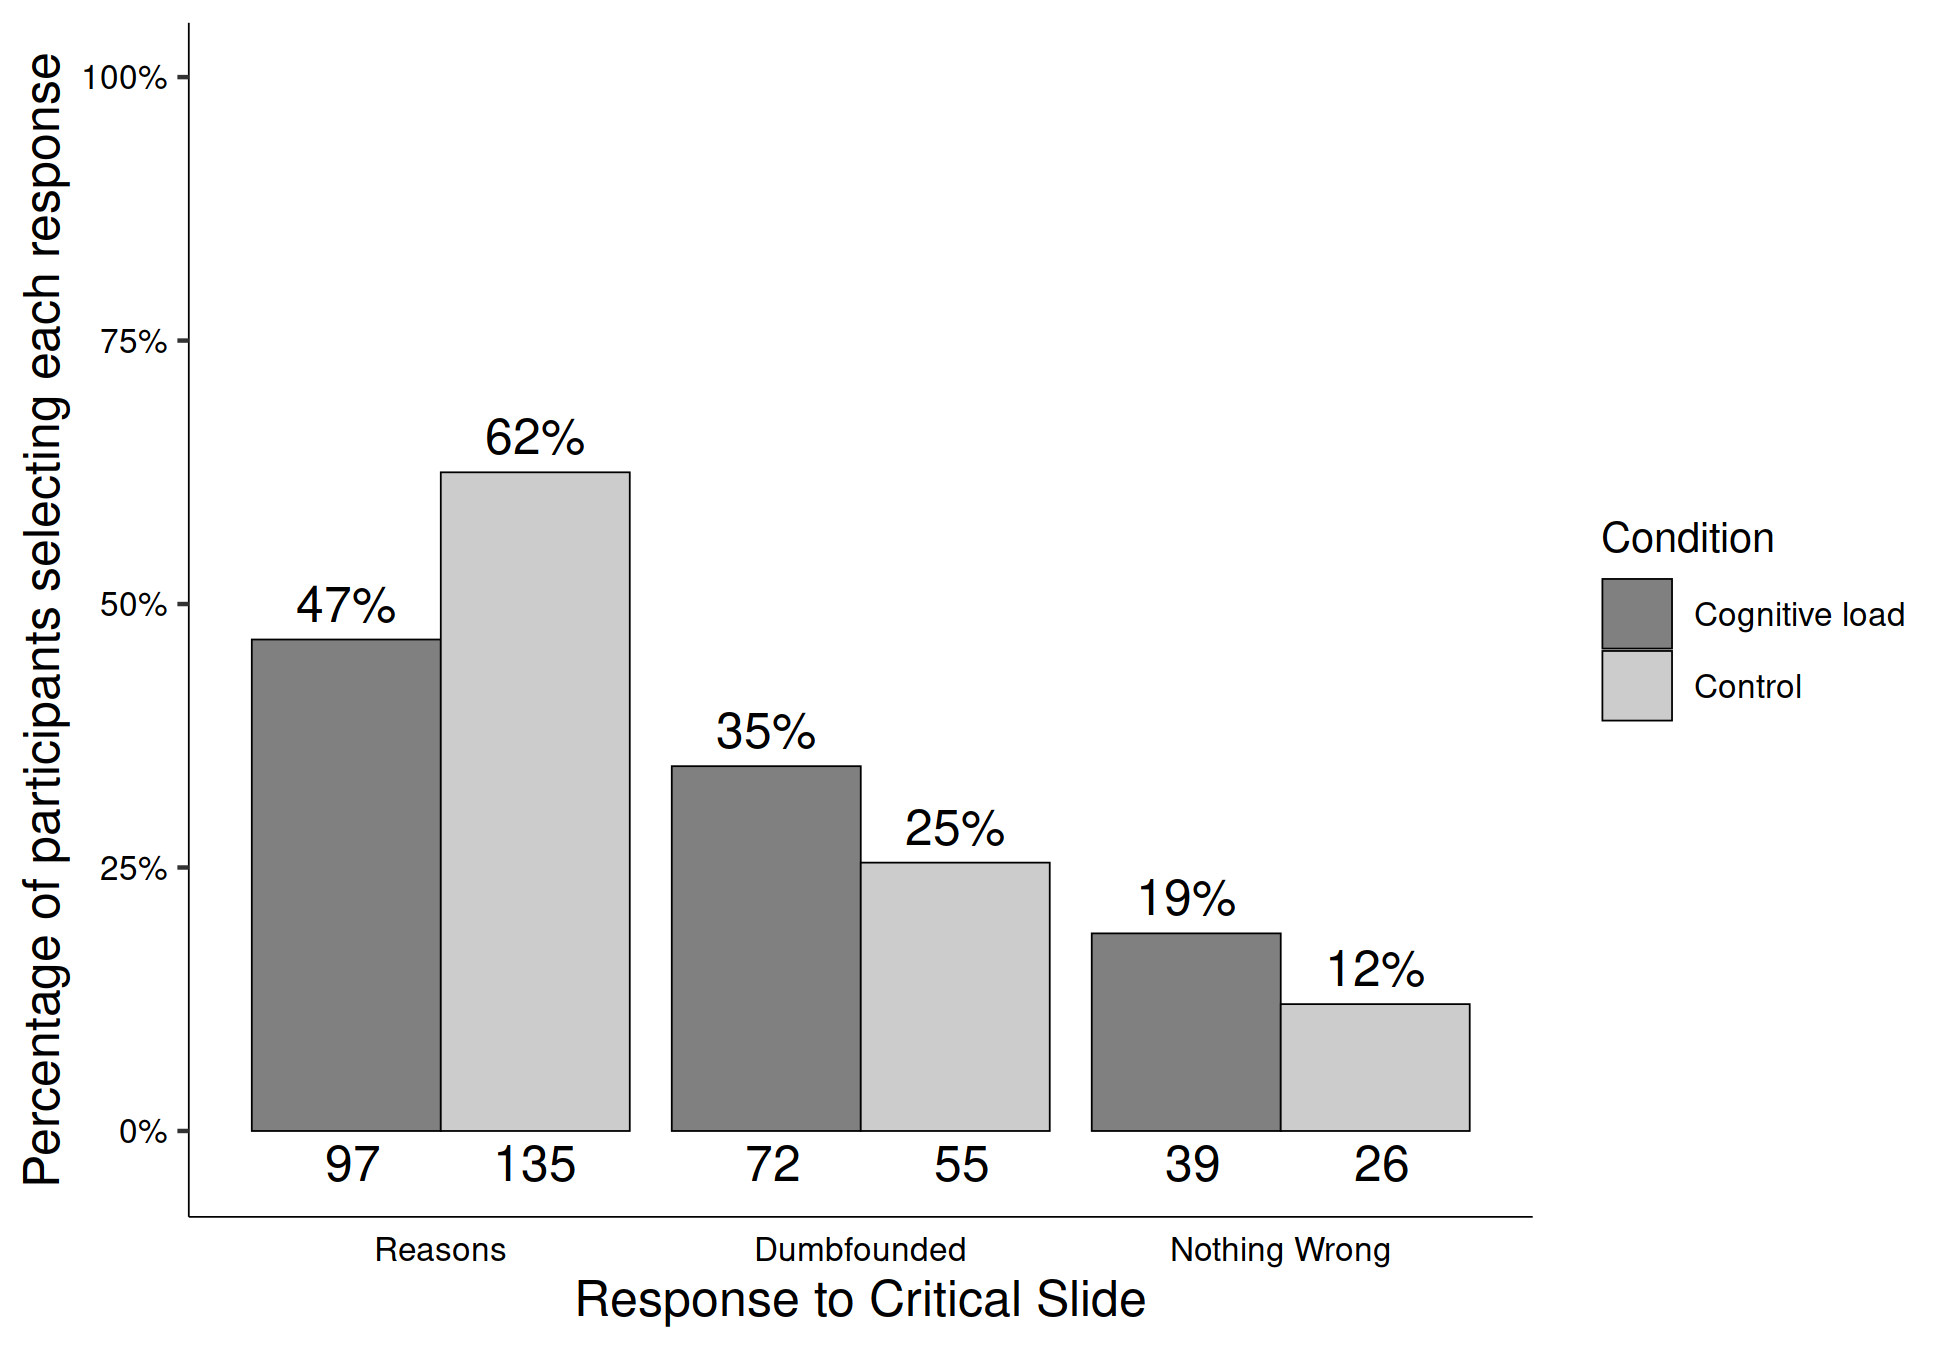
\includegraphics{Supplementary_files/figure-latex/figS6ch5S6fig2criticalconditionbTrolley-1} \caption{Study 6: Responses to critical slide depending on cognitive load (Trolley)}\label{fig:figS6ch5S6fig2criticalconditionbTrolley}
\end{figure}

\begin{figure}[!p]
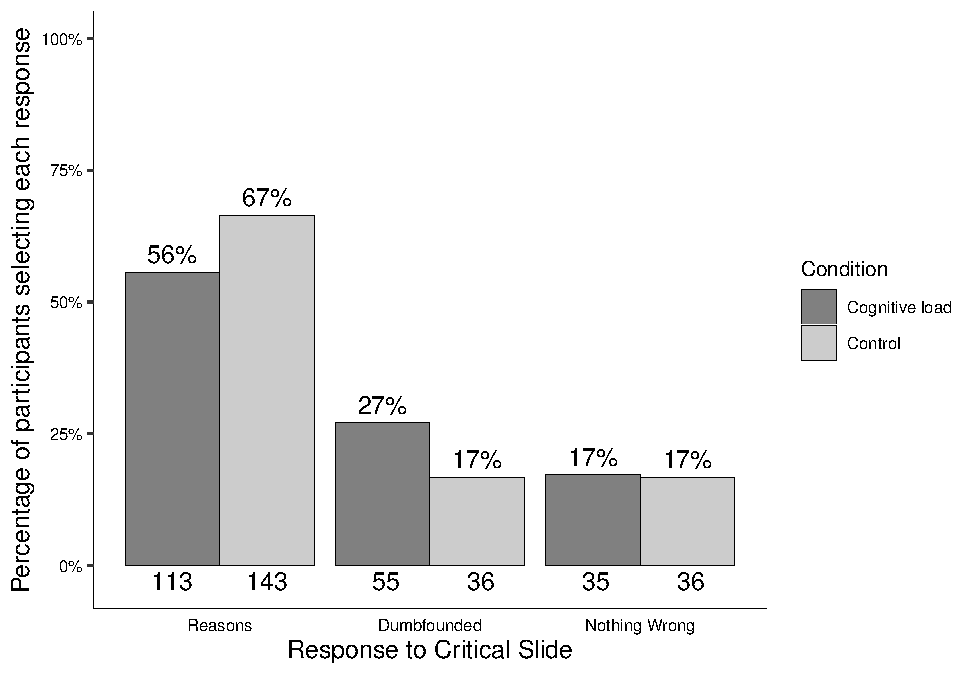
\includegraphics{Supplementary_files/figure-latex/figS6ch5S6fig2criticalconditionbHeinz-1} \caption{Study 6: Responses to critical slide depending on cognitive load (Heinz)}\label{fig:figS6ch5S6fig2criticalconditionbHeinz}
\end{figure}


\clearpage
\renewcommand{\listfigurename}{Figure captions}

\clearpage
\renewcommand{\listtablename}{Table captions}


\end{document}
